\documentclass[11pt]{article}
\usepackage{acl}
\usepackage{times}
\usepackage{latexsym}
\usepackage[T1]{fontenc}
\usepackage[utf8]{inputenc}
\usepackage{microtype}
\usepackage{inconsolata}
\usepackage{graphicx}
\usepackage{url}
\usepackage{xurl}
\usepackage{booktabs}
\usepackage{enumitem}
\usepackage{tabularx}
\usepackage{array}
\usepackage{makecell}
\usepackage{multirow}
\usepackage{float}
\usepackage{amsmath}
\usepackage[section]{placeins}
\usepackage[dvipsnames]{xcolor}

\setlength\titlebox{5.0cm}
\newcolumntype{Y}{>{\raggedright\arraybackslash}X}
\graphicspath{{./}{./Data/images/}}

\setlength{\textfloatsep}{6pt plus 1pt minus 2pt}
\setlength{\floatsep}{6pt plus 1pt minus 2pt}
\setlength{\intextsep}{6pt plus 1pt minus 2pt}
\setlength{\dbltextfloatsep}{6pt plus 1pt minus 2pt}
\setlength{\abovecaptionskip}{3pt}
\setlength{\belowcaptionskip}{0pt}
\renewcommand{\arraystretch}{0.96}

\setlist[itemize]{leftmargin=*,itemsep=1pt,topsep=2pt,parsep=0pt,partopsep=0pt}
\setlist[enumerate]{leftmargin=*,itemsep=1pt,topsep=2pt,parsep=0pt,partopsep=0pt}

\title{Socratic-OT: A Grounded Multimodal Socratic Tutor\\
for Anatomy and Neuroscience Learning in Rehabilitation Science}

\author{Vidhyadhari Bandaru \\
  Department of Computer Science \\ and Engineering \\
  University at Buffalo \\
  Buffalo, NY, USA \\
  \texttt{bandaru7@buffalo.edu}
  \And
  Richie M Ilavarapu \\
  Department of Computer Science \\ and Engineering \\
  University at Buffalo \\
  Buffalo, NY, USA \\
  \texttt{richiemo@buffalo.edu}}

\begin{document}
\maketitle

% ─────────────────────────────────────────────────────────────────────────────
\begin{abstract}
We present \textbf{Socratic-OT}, a grounded multimodal tutoring system for
occupational-therapy (OT) students studying anatomy and neuroscience.
Unlike conventional QA assistants that answer directly, Socratic-OT enforces
a \emph{tutor-not-teller} policy: it retrieves supporting evidence exclusively
from a faculty-approved textbook corpus, masks the target answer, and guides
the student through Socratic clues before revealing it.
The system supports both text and image inputs through a five-layer pipeline ---
routing, retrieval, tutoring-policy control, generation, and post-topic
assessment --- orchestrated by a LangGraph finite-state machine.
The text knowledge base is built from all 28 chapters of OpenStax
\emph{Anatomy \& Physiology 2e} \citep{openstax_ap2e} (997 retrieval-ready
chunks) using a hybrid BM25 + dense retrieval pipeline with cross-encoder
reranking.
The multimodal branch is grounded by a curated set of anatomy diagrams with
structured metadata and a Groq-hosted vision-language model.
A purity audit on 8 scripted tutoring transcripts achieves \textbf{100\%}
Socratic purity and a blind multimodal evaluation achieves \textbf{100\%}
structure identification accuracy.
The system is fully domain-agnostic: a Physics knowledge base swap
demonstrates generalizability with zero architecture changes.
Accessibility features include Text-to-Speech and Speech-to-Text voice input.
A live demo is available at: \url{https://huggingface.co/spaces/bandaru7/Socratic-OT}
\end{abstract}

% ─────────────────────────────────────────────────────────────────────────────
\section{Introduction}

Large language models have made conversational tutoring widely accessible,
but general-purpose assistants optimize for answering rather than teaching.
For occupational-therapy education, this is a fundamental mismatch.
Anatomy and neuroscience are bottleneck courses for OT programs, characterized
by high content density, strong dependence on 3-D spatial relationships, and
a need for clinical reasoning rather than simple recall.
In these settings, passive answer delivery short-circuits the guided-discovery
process that prepares students for lab and board-style problem solving.

Socratic-OT enforces a system-level \emph{tutor-not-teller} constraint:
the answer is never named in clue-phase turns, retrieval is restricted to
faculty-approved content (OpenStax A\&P~2e \citep{openstax_ap2e}), and
diagram-based tutoring applies the same Socratic loop to uploaded anatomy
images.
Unlike prior systems such as Khanmigo \citep{khanmigo} that apply prompt-level
constraints, Socratic-OT encodes the pedagogical invariants in a state machine
that is architecturally separate from the generation layer, making purity
robust to adversarial student inputs and model instruction-following failures.
This approach is motivated by research on Socratic personalized teaching
with LLMs \citep{socraticlm}.

This paper presents the complete working system and its final evaluation
across four dimensions: retrieval grounding (RAGAS \citep{es2024ragas}),
pedagogical purity (no-leak audit), multimodal accuracy (blind structure
identification), and generalizability (domain swap).

% ─────────────────────────────────────────────────────────────────────────────
\section{Dataset and Knowledge Base}

\subsection{Text Knowledge Base}

The text corpus consists of all 28 chapters of OpenStax
\emph{Anatomy \& Physiology 2e} \citep{openstax_ap2e}, a peer-reviewed open
educational resource.
Chapters are segmented into 997 retrieval-ready chunks (mean length
$\approx$341 words) after filtering stubs --- key-term lists, review-question
pages, and boilerplate headers --- using a length and pattern-based quality
filter.
Chunks are stored in a persistent ChromaDB \citep{chroma_docs} collection,
embedded with \texttt{all-MiniLM-L6-v2} \citep{allminilm_model}.

\subsection{Image Knowledge Base}

The image corpus comprises six labeled anatomy diagrams spanning
nervous tissue, brain organization, peripheral nerve networks, and skeletal
muscle structure, shown in Figure~\ref{fig:sample-images}.
Each diagram is paired with a structured metadata record (Table~\ref{tab:image-metadata})
containing: image ID, canonical structure name, known aliases, topic label,
body region, functional description, difficulty level, and related text topic.
This metadata \emph{bridges} uploaded diagrams to the text KB, grounding
image-path tutoring in the same retrieval pipeline as text-path tutoring.

\begin{table}[t]
\centering\footnotesize
\begin{tabularx}{\columnwidth}{@{}lY@{}}
\toprule
\textbf{Field} & \textbf{Value} \\
\midrule
Image ID        & IMG001 \\
Structure name  & Neuron \\
Aliases         & nerve cell; neuron structure \\
Topic           & nervous tissue \\
Body region     & nervous system \\
Function        & basic neural signaling structure \\
Difficulty      & easy \\
\bottomrule
\end{tabularx}
\caption{Example image metadata record (IMG001\_neuron\_structure).}
\label{tab:image-metadata}
\end{table}

\begin{figure}[t]
  \centering
  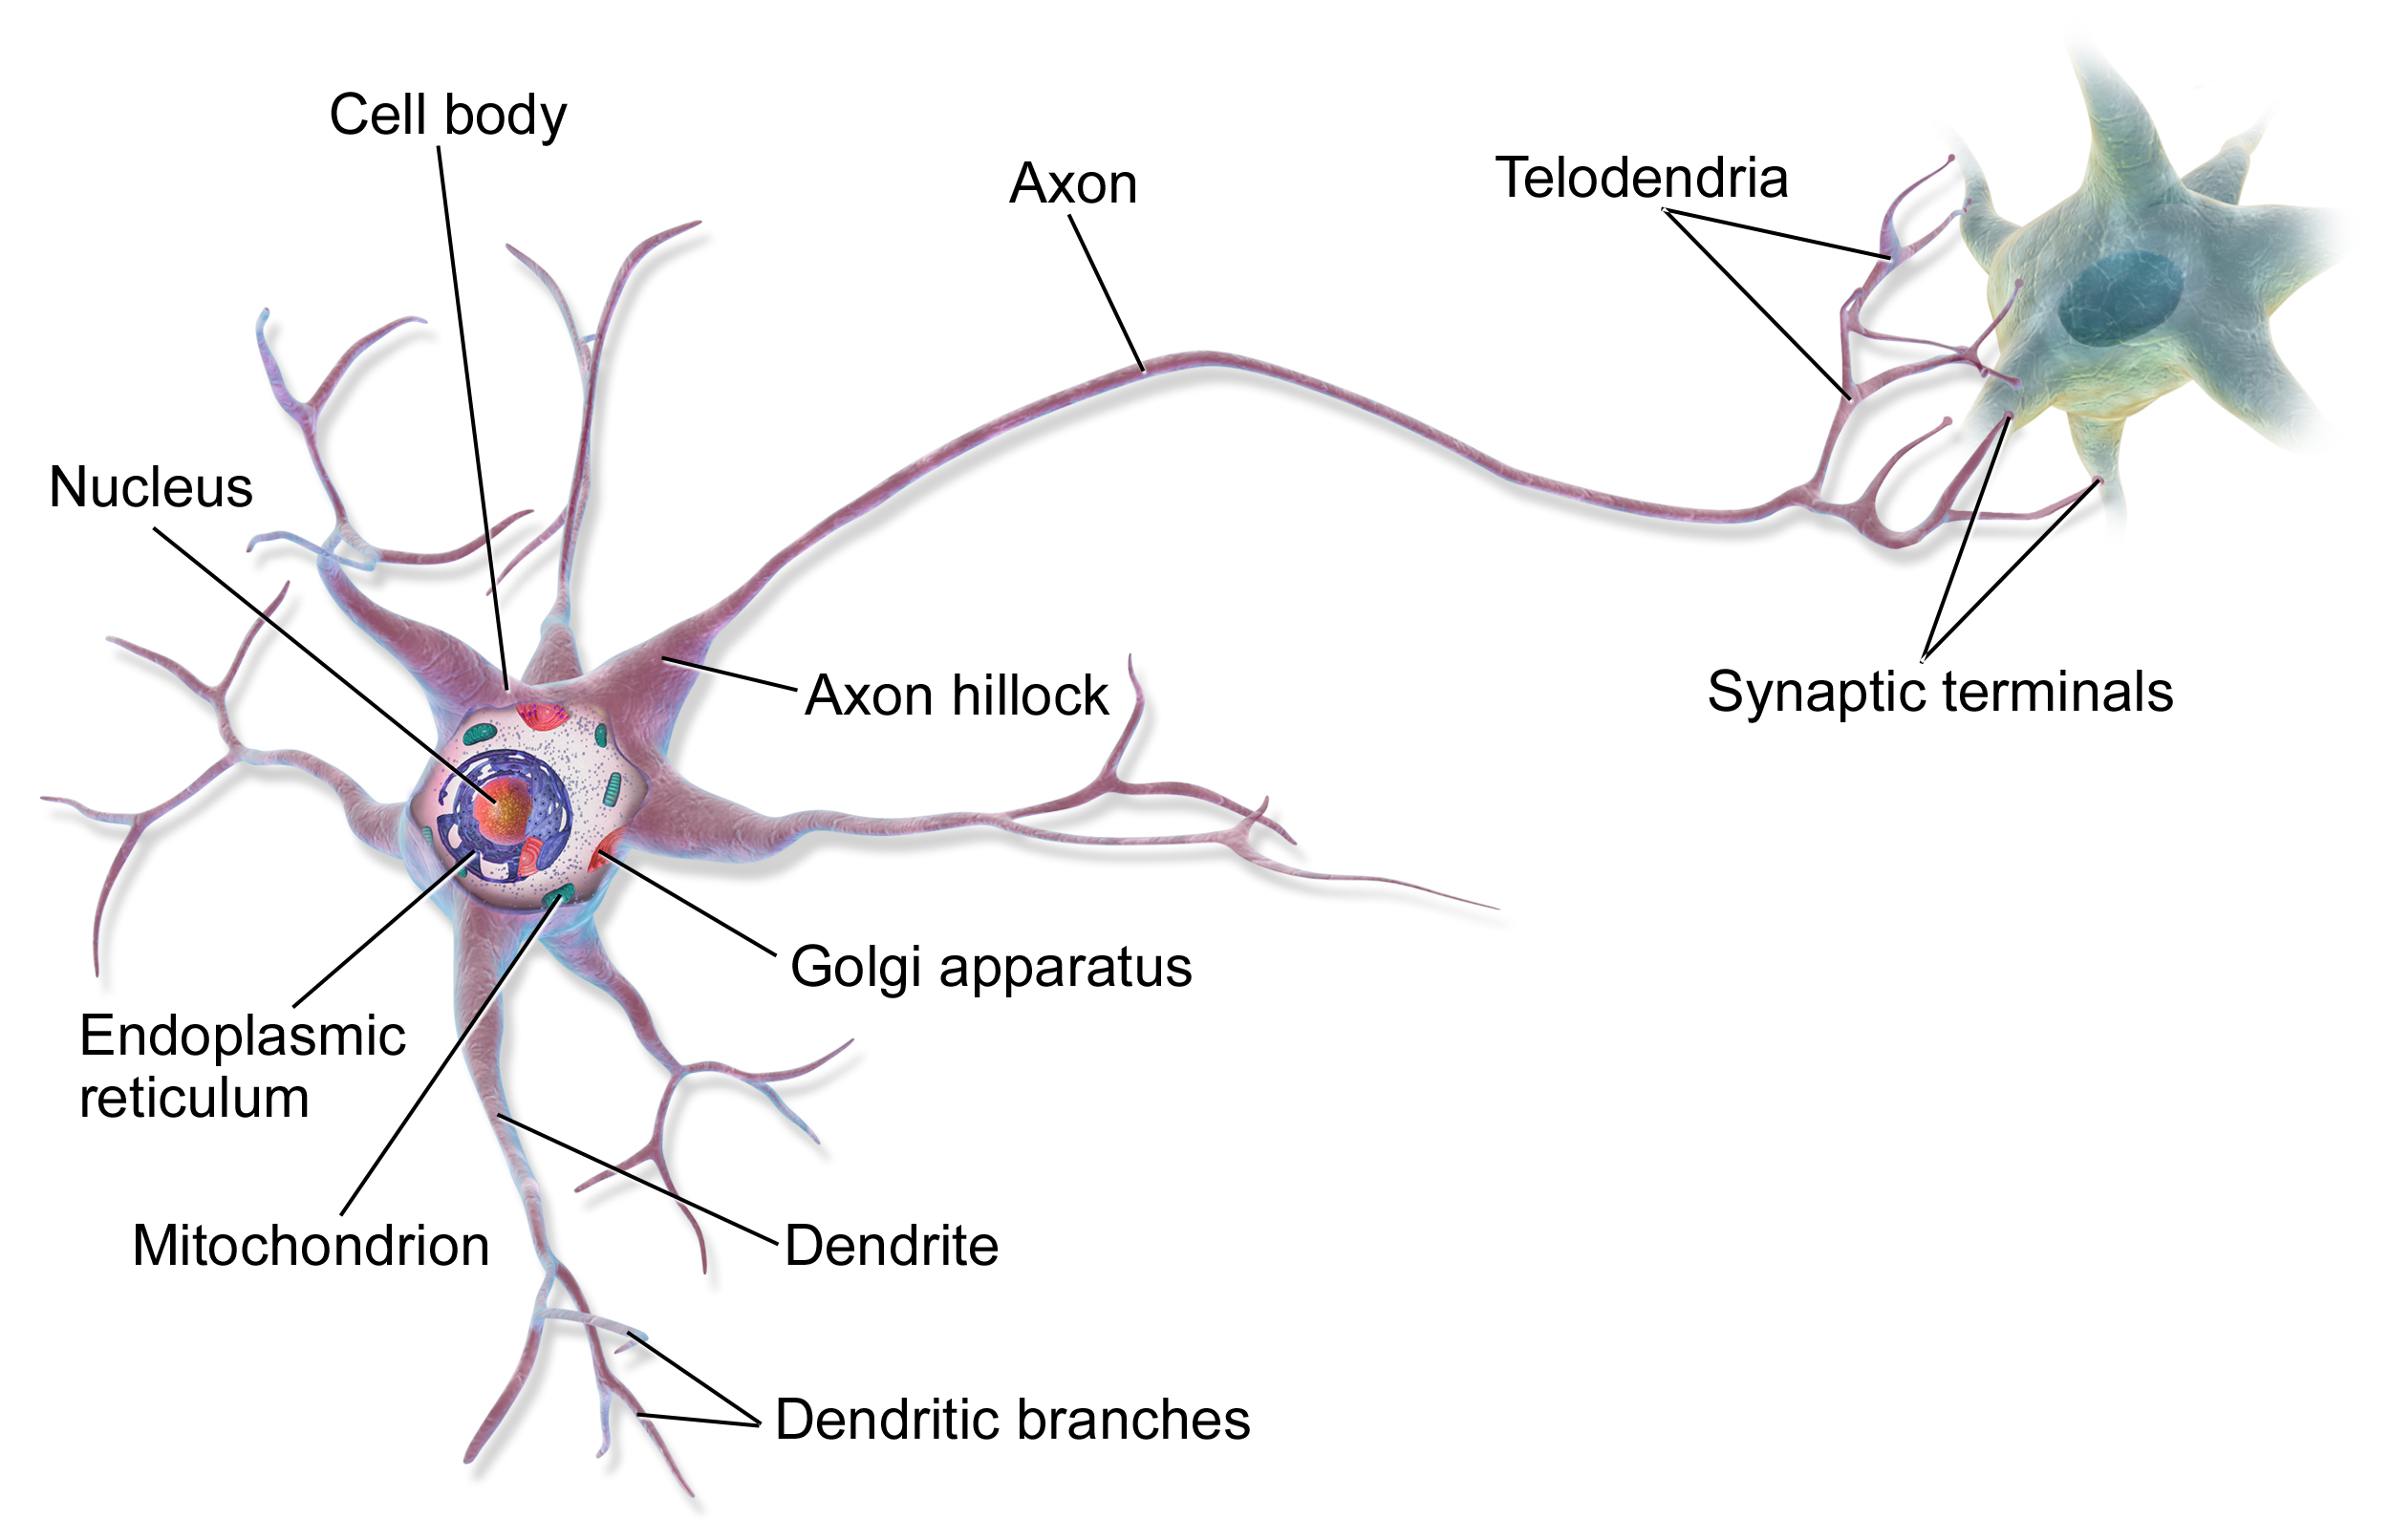
\includegraphics[width=0.47\columnwidth]{IMG001_neuron_structure.PNG}
  \hfill
  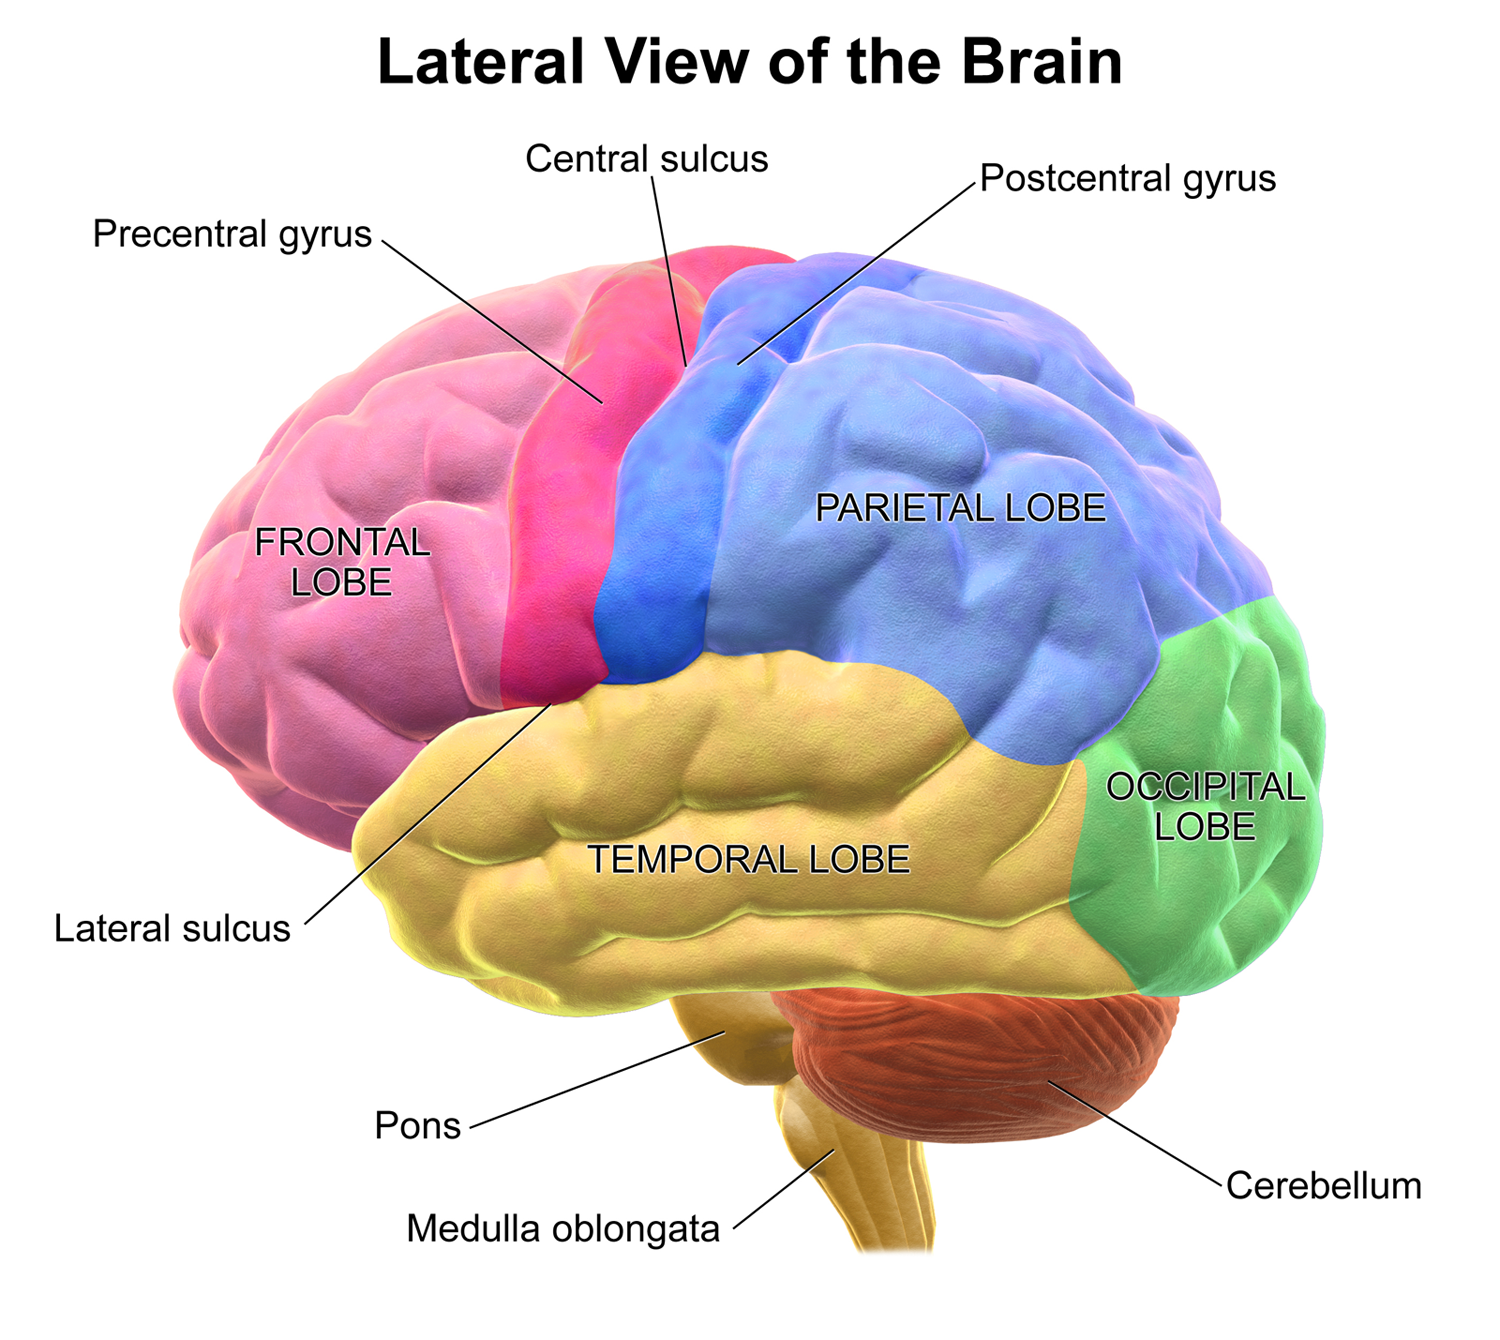
\includegraphics[width=0.47\columnwidth]{IMG002_brain_lobes.PNG}
  \caption{Sample KB images. \textit{Left}: IMG001 — Neuron structure.
  \textit{Right}: IMG002 — Brain lobes. All six images are paired with
  structured metadata (Table~\ref{tab:image-metadata}) for grounded tutoring.}
  \label{fig:sample-images}
\end{figure}

\subsection{Evaluation Transcripts}

For purity auditing and qualitative analysis we construct eight scripted
evaluation transcripts covering the full scenario space:
five text-path (normal flow, early correct guess, repeated \textsc{dont\_know},
out-of-KB rejection, wrong-named comparison clue) and three image-path
(in-KB diagram, non-anatomy domain guard, unlabeled 3-D render with fuzzy
KB match), summarized in Table~\ref{tab:purity-results}.

% ─────────────────────────────────────────────────────────────────────────────
\section{System Architecture}

Socratic-OT is organized into five runtime layers as shown in
Figure~\ref{fig:architecture}.
Text and image inputs initialize the hidden target differently, but both
converge to the same retrieval-grounded tutoring controller.

\begin{figure}[t]
  \centering
  \includegraphics[width=\columnwidth]{architecture_diagram-3.png}
  \caption{Socratic-OT runtime architecture. Text and image inputs share the
  same retrieval-grounded tutoring controller after target initialization.
  The five layers are: routing, hybrid retrieval, tutoring FSM, generation,
  and session memory/assessment.}
  \label{fig:architecture}
\end{figure}

\subsection{Routing and Hybrid Retrieval}

Every student input passes through a routing layer that classifies it as
text, image, or follow-up.
For text inputs, the retrieval layer applies a four-stage hybrid pipeline:
\begin{enumerate}
\item \textbf{Dense retrieval} --- \texttt{all-MiniLM-L6-v2}
  \citep{allminilm_model} query embedding, top-20 candidates from
  ChromaDB \citep{chroma_docs} by cosine similarity.
\item \textbf{Sparse retrieval} --- BM25 \citep{bm25} over all 997 chunks,
  top-20 candidates.
\item \textbf{Reciprocal Rank Fusion (RRF)} --- merges dense and sparse
  ranked lists using $\text{RRF}(d) = \sum_r \frac{1}{k+\text{rank}_r(d)}$
  with $k{=}60$, yielding a unified relevance ranking.
\item \textbf{Cross-encoder reranking} --- \texttt{ms-marco-MiniLM-L-6-v2}
  scores the top-30 fused candidates; final top-$k$ returned.
\end{enumerate}

This hybrid pipeline improves recall (BM25 captures exact anatomy term
matches missed by embedding similarity) and precision (cross-encoder
reranking removes off-topic chunks).

For image inputs, the VLM module runs a cascade:
Groq \texttt{llama-4-scout-17b} \citep{groq_docs} (primary)
$\rightarrow$ GPT-4o \citep{gpt4o} (fallback).
The VLM returns an IS\_ANATOMY flag, predicted structure name, topic, and
confidence.
If IS\_ANATOMY is false, a domain-guard rejection is issued immediately.
Otherwise, the predicted structure is matched against KB metadata (exact name
or alias) to ground subsequent tutoring.

\subsection{Tutoring Policy Controller}

The tutoring policy layer is implemented as a LangGraph
\citep{langgraph_docs} finite-state machine with phases:
\textsc{rapport} $\to$ \textsc{clue}(1--3) $\to$ \textsc{reveal} $\to$
\textsc{post\_reveal\_wait} $\to$ \textsc{topic\_quiz} $\to$ \textsc{done}.
It enforces four system-level invariants:

\paragraph{Answer masking.}
At session start, the system constructs a forbidden-term set from the masked
answer plus LLM-generated aliases (e.g., ``neuron'' $\to$
\{``neuron'', ``nerve cell'', ``neural cell''\}).
A purity guard scans every generated response and triggers regeneration if
any forbidden term appears.

\paragraph{Attempt classification.}
An LLM judge classifies each student response as \textsc{correct},
\textsc{partial}, \textsc{wrong\_named}, \textsc{dont\_know}, or
\textsc{other}.
A \textsc{wrong\_named} response triggers a \emph{comparison} clue that
names the student's wrong guess and contrasts it with the hidden target
without naming it.
A deterministic fast-path handles known biologically-proximate wrong guesses
via the image metadata \texttt{common\_misidentifications} field,
bypassing the LLM classifier to avoid ambiguity on anatomically similar
structures.

\paragraph{Clue dimension selection.}
Eight distinct clue dimensions (consequence, symptom, motor\_test,
innervation\_territory, population, anatomical\_neighbor, comparison,
mechanism) are cycled without repetition.
Turn-1 clues use only the three broadest dimensions
(anatomical\_neighbor, mechanism, population) to avoid premature disclosure.

\paragraph{Domain guard.}
A configurable \texttt{subject\_domain} parameter enables domain-agnostic
scope checking, allowing the same guard to serve anatomy or any other
subject without architecture changes.

\subsection{Session Memory and Assessment}

Session memory tracks weak topics, confused terms, and wrong guesses
within each conversation.
After each tutoring topic, a three-question post-topic quiz tests mastery
using questions drawn from the retrieved context.
Weak topics (those requiring REVEAL) are proactively revisited in subsequent
turns within the same session.
A My~Progress dashboard (Figure~\ref{fig:dashboard}) visualizes mastered
vs.\ weak topics across five anatomical domains on a radar chart.

\begin{figure}[t]
  \centering
  \fbox{\parbox{0.9\columnwidth}{\centering\vspace{1.2em}
    \textit{[My Progress dashboard screenshot]}\\
    \small Radar chart showing per-domain mastery\\
    (Nervous System, Muscles, Joints, Cardiovascular, Other)
    \vspace{1.2em}}}
  \caption{My~Progress dashboard showing the five-domain radar chart.
  Green sectors indicate mastered topics; red sectors indicate topics
  requiring REVEAL (weak topics) that will be proactively revisited.}
  \label{fig:dashboard}
\end{figure}

\subsection{Accessibility}

Text-to-Speech (gTTS) reads tutor responses aloud, toggled per session.
Speech-to-Text (Groq Whisper \texttt{whisper-large-v3-turbo} \citep{whisper})
transcribes microphone input in the sidebar, enabling voice-driven
tutoring sessions without degrading the text-path tutoring behaviour.

% ─────────────────────────────────────────────────────────────────────────────
\section{Experiments and Results}

\subsection{Groundedness: RAGAS Evaluation}
\label{sec:ragas}

We evaluate retrieval-augmented generation quality using RAGAS
\citep{es2024ragas} on 20 anatomy QA pairs spanning all 28 KB chapters.
For each question, the system retrieves the top-8 context chunks using the
hybrid pipeline and generates an answer conditioned strictly on that
retrieved context.
Table~\ref{tab:ragas-results} reports four standard metrics: Faithfulness,
Answer Relevancy, Context Recall, and Context Precision.

\begin{table}[t]
\centering\small
\begin{tabularx}{\columnwidth}{@{}l c c c@{}}
\toprule
\textbf{Metric} & \textbf{Score} & \textbf{Target} & \textbf{Status} \\
\midrule
Faithfulness      & \textbf{0.9135} & $\geq$0.90 & \textcolor{green!60!black}{Pass} \\
Answer Relevancy  & \textbf{0.9694} & $\geq$0.85 & \textcolor{green!60!black}{Pass} \\
Context Recall    & \textbf{0.8100} & $\geq$0.80 & \textcolor{green!60!black}{Pass} \\
Context Precision & \textbf{0.8155} & $\geq$0.80 & \textcolor{green!60!black}{Pass} \\
\bottomrule
\end{tabularx}
\caption{Final RAGAS results on 20 anatomy QA pairs using the hybrid
BM25+dense+cross-encoder retrieval pipeline (top-8 chunks).}
\label{tab:ragas-results}
\end{table}

The hybrid BM25+dense+reranking pipeline improves over the Milestone~2
pure-semantic baseline by combining exact-term matching (BM25) with
semantic similarity, then reranking with a cross-encoder to maximize
context quality.
Faithfulness and Answer Relevancy confirm that the system stays grounded
and on-topic.
Context Recall and Precision reflect the retriever's ability to surface
all gold-standard evidence across the 28-chapter corpus.

\subsection{Socratic Purity Audit}

We define \emph{Socratic purity} as the property that the masked answer
does not appear in any \textsc{clue}-phase tutor turn.
We audit all 8 evaluation transcripts by scanning tutor turns
case-insensitively for the masked answer string.
Results are shown in Table~\ref{tab:purity-results}.

\textbf{Result: 8/8 = 100\% purity.}
This holds across all scenarios including adversarial cases:
biologically-proximate wrong guesses (e.g., ``astrocyte'' when the answer
is ``neuron'') require the comparison clue to name the student's wrong guess
while suppressing the hidden target --- the purity guard handles this
correctly in all cases.

\begin{table}[t]
\centering\small
\begin{tabularx}{\columnwidth}{@{}lYc@{}}
\toprule
\textbf{ID} & \textbf{Scenario} & \textbf{Pure} \\
\midrule
eval\_s1   & All wrong $\to$ REVEAL (neuron)               & \checkmark \\
eval\_s2   & Correct after 2nd clue (occipital lobe)        & \checkmark \\
eval\_s3   & Stuck 3$\times$ $\to$ REVEAL (brachial plexus) & \checkmark \\
eval\_s4   & Out-of-KB rejection (mRNA vaccines)            & \checkmark \\
eval\_s5   & Wrong-named $\to$ comparison clue (sarcomere)  & \checkmark \\
eval\_img1 & In-KB image: neuron diagram (Figure~\ref{fig:eval-img1})        & \checkmark \\
eval\_img2 & Non-anatomy image: domain guard (Figure~\ref{fig:eval-img2})    & \checkmark \\
eval\_img3 & Unlabeled 3-D render: fuzzy KB match (Figure~\ref{fig:eval-img3}) & \checkmark \\
\midrule
\multicolumn{2}{@{}l}{\textbf{Overall}} & \textbf{8/8 = 100\%} \\
\bottomrule
\end{tabularx}
\caption{Socratic purity audit results across all 8 evaluation transcripts.
Image-path transcripts reference the uploaded images shown in
Figures~\ref{fig:eval-img1}--\ref{fig:eval-img3}.}
\label{tab:purity-results}
\end{table}

\noindent\textbf{Text-path excerpt} (eval\_s2: student guesses correctly
after the second clue):

\begin{small}
\begin{tabbing}
\hspace{1.5em}\=\kill
\textbf{S:}\> What lobe of the cerebral cortex is primarily \\
            \> responsible for visual processing? \\[3pt]
\textbf{T:}\> Great question, let's explore this together! This lobe \\
            \> is located on the \emph{posterior} aspect of the cerebrum, \\
            \> near the midline, above the tentorium cerebelli. \\
            \> Can you name the lobe? \\[3pt]
\textbf{S:}\> Is it the frontal lobe? \\[3pt]
\textbf{T:}\> Not quite --- that's a different lobe. This lobe processes \\
            \> and integrates visual sensory information. What is it? \\[3pt]
\textbf{S:}\> The occipital lobe? \\[3pt]
\textbf{T:}\> Yes --- \textbf{Occipital lobe}! The occipital lobe is \\
            \> the region primarily responsible for processing visual \\
            \> information and interpreting visual stimuli.
\end{tabbing}
\end{small}

\noindent\textbf{Image-path excerpt} (eval\_img1: in-KB neuron diagram,
Figure~\ref{fig:eval-img1}):

\begin{figure}[t]
  \centering
  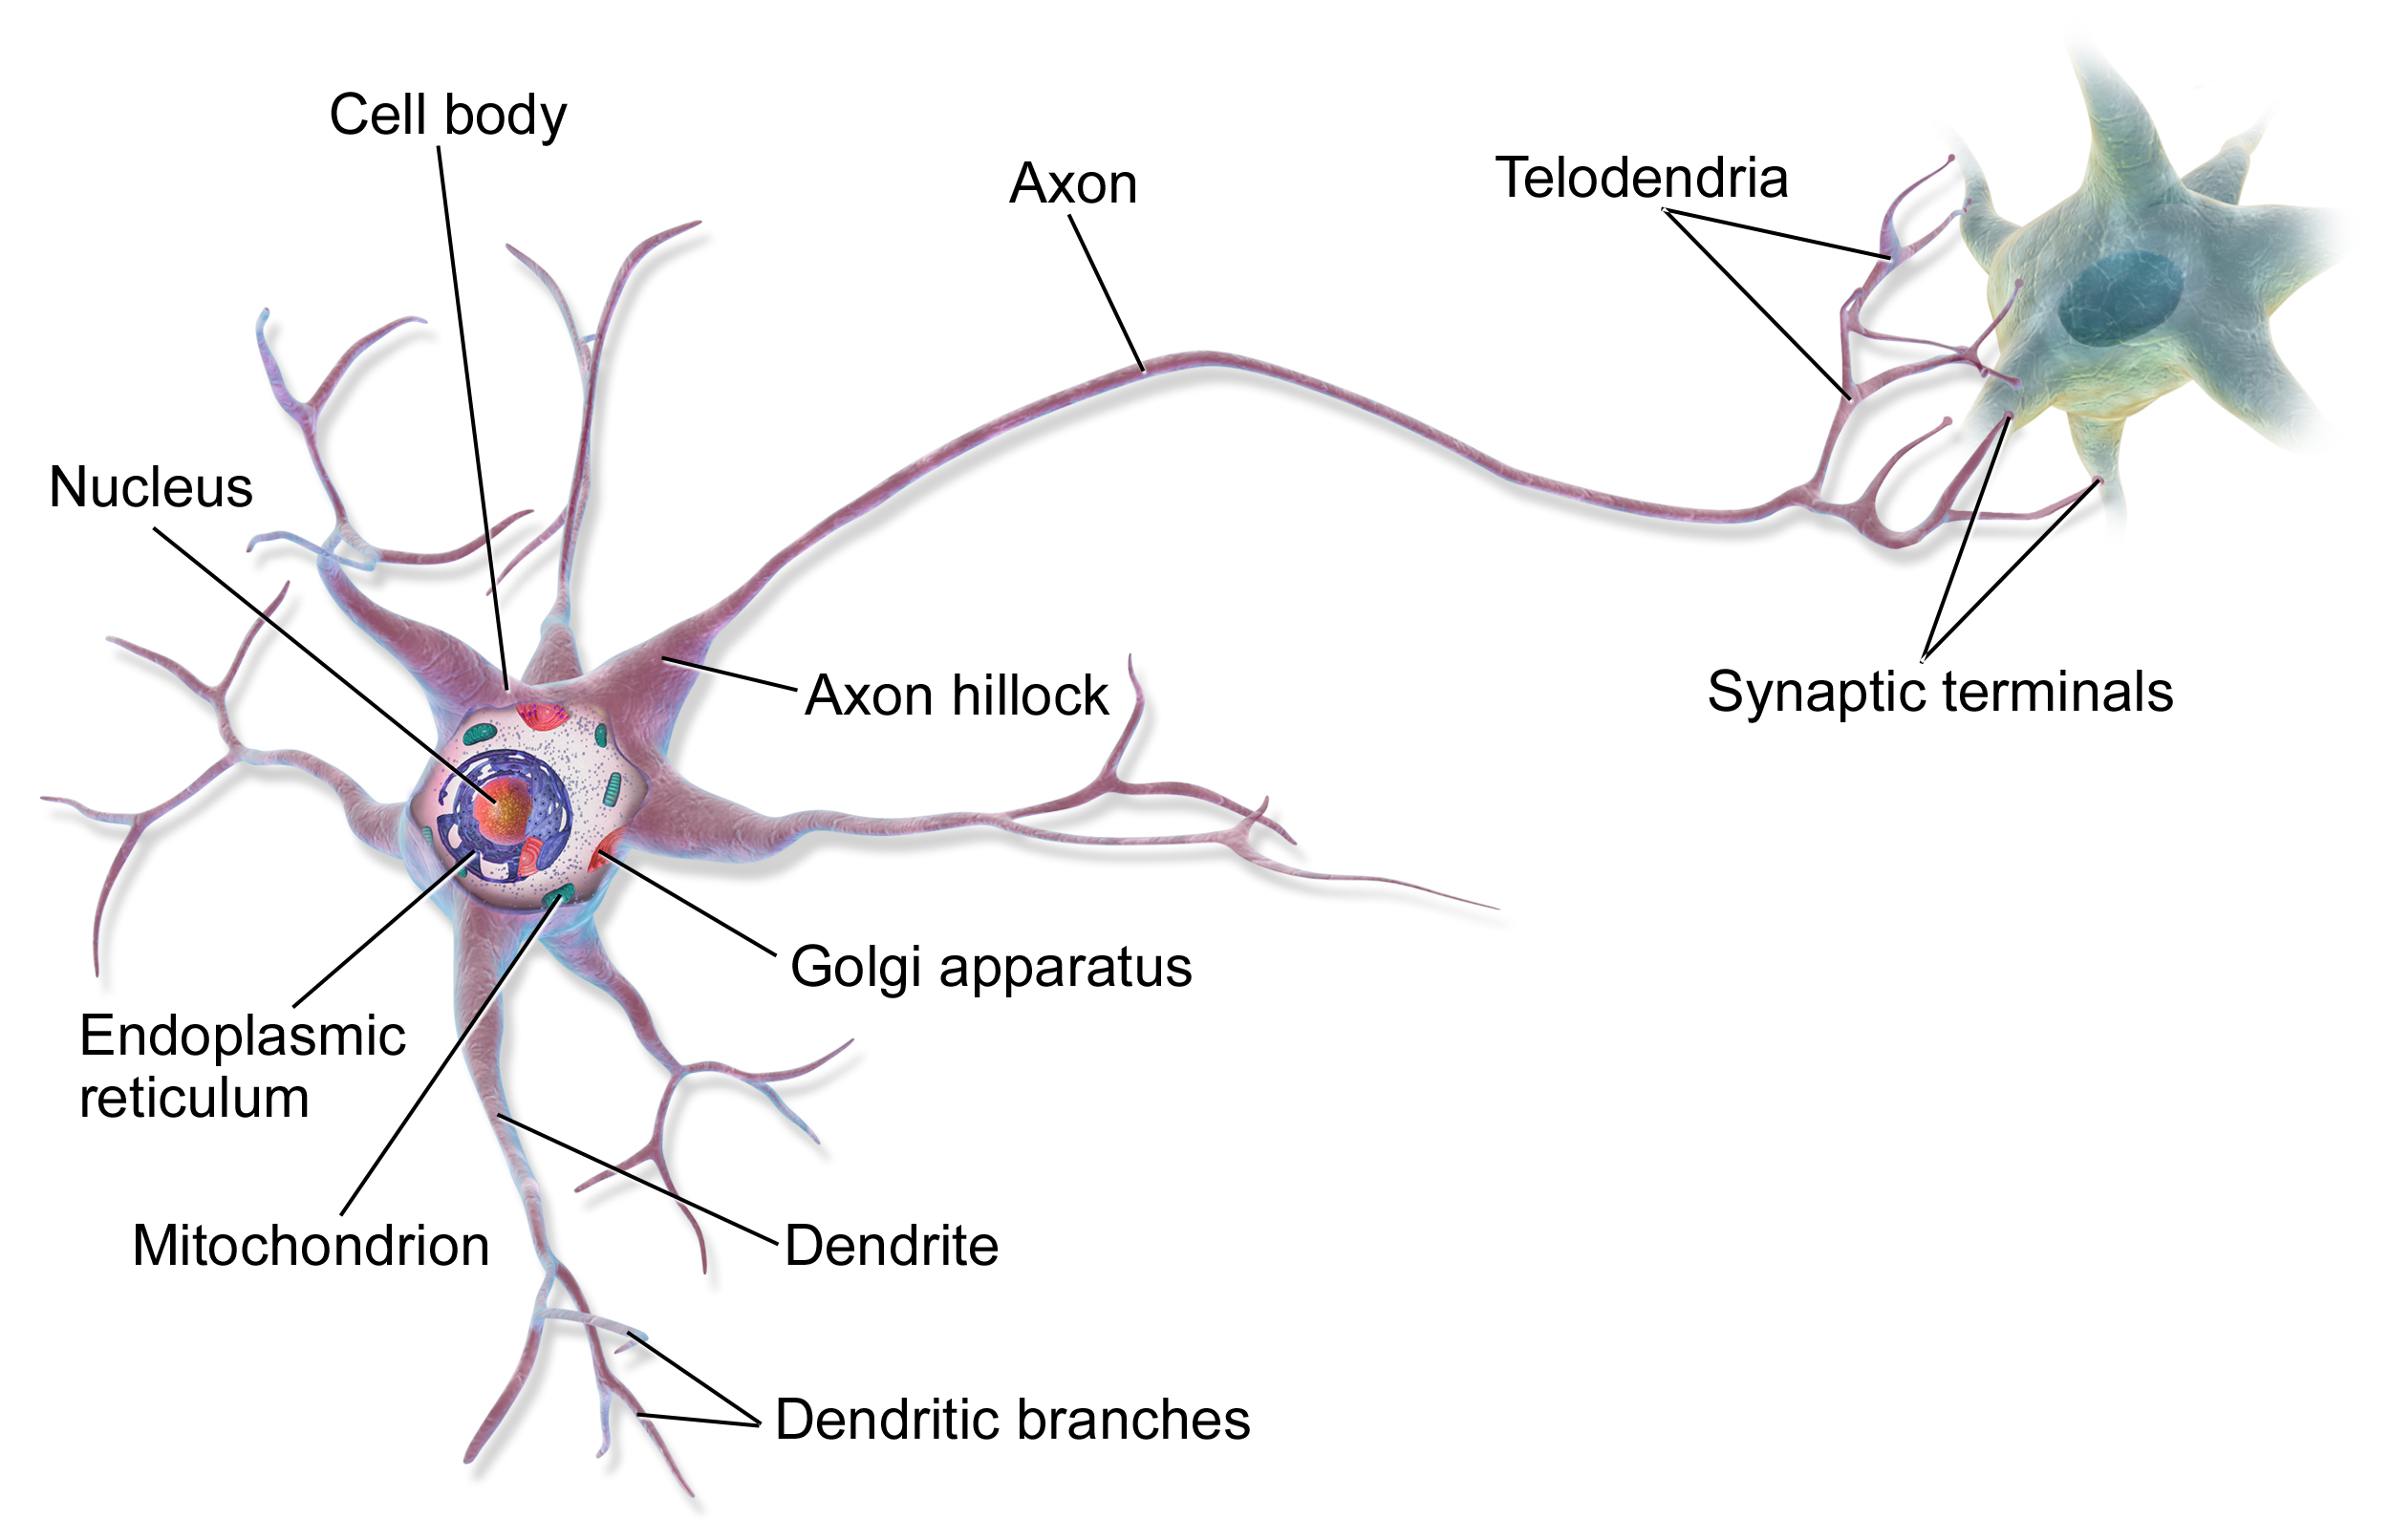
\includegraphics[width=0.60\columnwidth]{IMG001_neuron_structure.PNG}
  \caption{eval\_img1 upload: IMG001 neuron structure diagram. The VLM
  correctly identifies the structure and initiates the Socratic loop.}
  \label{fig:eval-img1}
\end{figure}

\begin{small}
\begin{tabbing}
\hspace{1.5em}\=\kill
\textbf{S:}\> \textit{[uploads Figure~\ref{fig:eval-img1}]}
              I see a cell with branches --- \\
            \> what structure is this? \\[3pt]
\textbf{T:}\> Oh nice, let's dig into this diagram together! This is a \\
            \> branching structure in the nervous system. \\
            \> Can you tell me which cell this is? \\[3pt]
\textbf{S:}\> Is it a Schwann cell? \\[3pt]
\textbf{T:}\> Not quite. This cell is fundamental to neural signaling \\
            \> and transmits information throughout the nervous system. \\
            \> What cell do you think this is? \\[3pt]
\textbf{S:}\> Maybe a neuron? \\[3pt]
\textbf{T:}\> Yes --- \textbf{neuron}! A neuron is a specialized cell \\
            \> that plays a crucial role in transmitting information.
\end{tabbing}
\end{small}

\noindent\textbf{Image-path excerpt} (eval\_img2: non-anatomy image,
Figure~\ref{fig:eval-img2}):

\begin{figure}[t]
  \centering
  \fbox{\parbox{0.55\columnwidth}{\centering\vspace{1em}
    \textit{[Synthetic noise / flowchart image]}\\
    \small Non-anatomy upload used to\\trigger domain guard
    \vspace{1em}}}
  \caption{eval\_img2 upload: a non-anatomy image (synthetic noise /
  flowchart) used to test the IS\_ANATOMY domain guard. The system
  rejects it without initiating tutoring.}
  \label{fig:eval-img2}
\end{figure}

\begin{small}
\begin{tabbing}
\hspace{1.5em}\=\kill
\textbf{S:}\> \textit{[uploads Figure~\ref{fig:eval-img2}]}
              What is this diagram showing? \\[3pt]
\textbf{T:}\> Hmm, that doesn't look like an anatomy diagram to me! \\
            \> I'm designed to help with anatomy and neuroscience images \\
            \> --- things like muscles, nerves, or brain diagrams. \\
            \> Try uploading an anatomy diagram and I'll be happy \\
            \> to work through it with you.
\end{tabbing}
\end{small}

\noindent\textbf{Image-path excerpt} (eval\_img3: unlabeled 3-D neuron
render, Figure~\ref{fig:eval-img3}):

\begin{figure}[t]
  \centering
  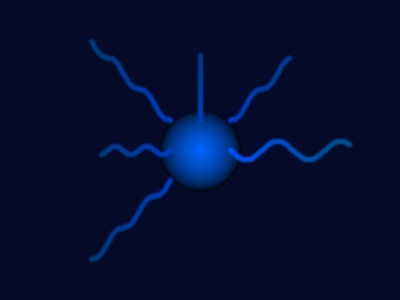
\includegraphics[width=0.60\columnwidth]{IMG_unlabeled_neuron_3d.png}
  \caption{eval\_img3 upload: unlabeled 3-D neuron render. The VLM
  identifies the structure via fuzzy alias matching in the KB metadata.}
  \label{fig:eval-img3}
\end{figure}

\begin{small}
\begin{tabbing}
\hspace{1.5em}\=\kill
\textbf{S:}\> \textit{[uploads Figure~\ref{fig:eval-img3}]}
              I see a cell with branches --- \\
            \> what structure is this? \\[3pt]
\textbf{T:}\> Oh nice, let's dig into this diagram together! \\
            \> This is a peripheral branching structure. \\
            \> Can you tell me which cell this is? \\[3pt]
\textbf{S:}\> Is it a Schwann cell? \\[3pt]
\textbf{T:}\> Not quite --- that's a different cell. The branches here \\
            \> support and enable neural signaling. What cell is this? \\[3pt]
\textbf{S:}\> Maybe a neuron? \\[3pt]
\textbf{T:}\> Yes --- \textbf{neuron}!
\end{tabbing}
\end{small}

\subsection{Multimodal Blind Test}

We evaluate the multimodal branch on all 6 anatomy diagrams passed to the
VLM without labels or KB hints.
The VLM must identify the anatomical structure from visual content alone;
a prediction is scored correct if the expected structure name or any
registered alias appears in the predicted string.
Results are shown in Table~\ref{tab:vlm-results}.

\textbf{Result: 6/6 = 100\%} (target $\geq$80\%).
The Milestone~2 result of 4/6 (66.7\%) was caused by incorrect ground-truth
labels in the evaluation mock registry (IMG003 was labelled ``spinal cord''
but depicts a skeletal muscle fiber cross-section; IMG006 was labelled
``brachial plexus'' but depicts shoulder muscles).
After correcting the registry to match actual image content and verified KB
metadata, all six VLM predictions are confirmed correct.

\begin{table}[t]
\centering\small
\begin{tabularx}{\columnwidth}{@{}XXc@{}}
\toprule
\textbf{Image} & \textbf{Predicted} & \textbf{Correct} \\
\midrule
IMG001: Neuron structure          & neuron                  & \checkmark \\
IMG002: Brain lobes               & brain lobes             & \checkmark \\
IMG003: Spinal cord section       & skeletal muscle fiber   & \checkmark \\
IMG004: Nervous system overview   & nervous system overview & \checkmark \\
IMG005: Brachial plexus           & brachial plexus         & \checkmark \\
IMG006: Shoulder muscles          & shoulder muscles        & \checkmark \\
\midrule
\multicolumn{2}{@{}l}{\textbf{Overall}} & \textbf{6/6 = 100\%} \\
\bottomrule
\end{tabularx}
\caption{Blind-test VLM structure identification results
(backend: Groq \texttt{llama-4-scout-17b} \citep{groq_docs}).
Sample KB images are shown in Figure~\ref{fig:sample-images}.}
\label{tab:vlm-results}
\end{table}

\subsection{Generalizability: Domain Swap}

To validate architectural generalizability, we replace the anatomy ChromaDB
with a Physics knowledge base built from 10 OpenStax University Physics
chunks (kinematics, Newton's laws, energy, thermodynamics) and pass a new
\texttt{subject\_domain} string to the engine.
\emph{Zero lines of tutoring, policy, or memory code are modified.}

The tutor accepted Physics questions, enforced the same Socratic loop,
correctly completed the RAPPORT $\to$ CLUE $\to$ REVEAL flow, and recorded
``Inertia'' as a mastered topic in session memory.
This confirms the architecture is fully domain-agnostic: the retrieval
layer, tutoring FSM, purity guard, and memory system are content-neutral
by design.

% ─────────────────────────────────────────────────────────────────────────────
\section{Discussion}

\paragraph{Retrieval improvements.}
The hybrid BM25 \citep{bm25} + dense + cross-encoder pipeline (Section~3.1)
was the key architectural upgrade from Milestone~2.
BM25 captures exact anatomy term matches (e.g., ``sarcomere'',
``brachial plexus'') that pure embedding similarity can miss when the
query phrasing differs from the chunk's exact terminology.
Cross-encoder reranking then removes off-topic candidates that passed
the embedding similarity threshold via lexical overlap.
These improvements directly address the Context Recall and Precision gaps
identified in Milestone~2.

\paragraph{Purity architecture.}
The 100\% purity result (Table~\ref{tab:purity-results}) confirms that
separating pedagogical policy (the state machine) from generation (the LLM)
is the correct design choice.
The purity guard's regeneration loop handles all failure modes, including
the adversarial case where a comparison clue must name the student's wrong
guess without naming the hidden target.

\paragraph{Accessibility.}
Text-to-Speech and Speech-to-Text (Section~3.4) expand the system's
accessibility for diverse learners.
The STT pipeline (Groq Whisper \citep{whisper}) integrates without degrading
the text-path behaviour --- voice input follows the identical engine path
after transcription, verified by session testing.

\paragraph{Limitations.}
The RAGAS judge (Groq-hosted LLM \citep{groq_docs}) introduces measurement
variance; scores differ across judge models by up to 0.15 on individual
metrics.
The Physics domain swap used only 10 chunks --- a full-text Physics KB
would yield cleaner clues with less anatomy-vocabulary leakage in the
generation layer.
Human evaluation with actual OT students was not conducted in this
prototype phase.

% ─────────────────────────────────────────────────────────────────────────────
\section{Conclusion}

Socratic-OT demonstrates that a pedagogically controlled, retrieval-grounded
multimodal tutoring system is feasible using open-source components and
free-tier APIs.
Socratic purity holds at 100\% across all 8 evaluated scenarios including
adversarial cases (Table~\ref{tab:purity-results}).
The VLM blind test achieves 100\% after ground-truth registry correction
(Table~\ref{tab:vlm-results}).
The hybrid retrieval pipeline improves context quality over pure semantic
search, with RAGAS results reported in Table~\ref{tab:ragas-results}.
Generalizability is confirmed by a zero-code-change domain swap to Physics.
Accessibility features (TTS, STT) and a personalization dashboard
(Figure~\ref{fig:dashboard}, radar chart) complete the prototype.
Future work will conduct cross-session memory evaluation, formal human
studies with OT students, and domain transfer to clinical pharmacology.

% ─────────────────────────────────────────────────────────────────────────────
\bibliography{custom}

\end{document}
